%----------------------------------------------------------------------------------------
%	PACKAGES AND THEMES
%----------------------------------------------------------------------------------------
\documentclass[aspectratio=43,xcolor=dvipsnames]{beamer}
\usetheme{SimplePlus}
\usepackage[utf8]{vietnam}
\usepackage{subfigure}
\usepackage{hyperref}
\usepackage{graphicx}
\usepackage{booktabs} 
\usepackage{amsmath}
%----------------------------------------------------------------------------------------
%	TITLE PAGE
%----------------------------------------------------------------------------------------
%[plain, noframenumbering]
\title[short title]{Thiết kế Database}
\subtitle{\Large{HUSTFood}}

\institute[HUST]
{
	Trường Công nghệ Thông tin và Truyền thông \\
	Đại học Bách Khoa Hà Nội
}
\date{Ngày 27 tháng 6 năm 2022}


%----------------------------------------------------------------------------------------
%	PRESENTATION SLIDES
%----------------------------------------------------------------------------------------

\begin{document}
	
	\begin{frame}[plain, noframenumbering]
		\titlepage
	\end{frame}
	\begin{frame}[plain, noframenumbering]{Thành viên trong nhóm}
		\begin{table}[!h]
			% \centering
			\label{ba2}
			\scalebox{1.2}{
				\begin{tabular}{|c|c|} \hline
					\textbf{Họ tên} & \textbf{MSSV}  \\ \hline 
					Phan Minh Anh Tuấn  & 20205227\\ 
					Nguyễn Thị Hoài Linh & 20205231\\ 
					Vũ Minh Long & 20200373\\ 
					Đàm Ngọc Khánh & 20205207\\ \hline 
				\end{tabular}
			}
		\end{table}
		% \begin{itemize}
			%     \item Phan Minh Anh Tuấn - 20205227
			%     \item Nguyễn Thị Hoài Linh - 20205231
			%     \item Vũ Minh Long - 20200373
			%     \item Đàm Ngọc Khánh - 20205207
			% \end{itemize}
	\end{frame}
	%------------------------------------------------
	\begin{frame}{Tổng quan Database}
		\begin{figure}[ht!]
			\centerline{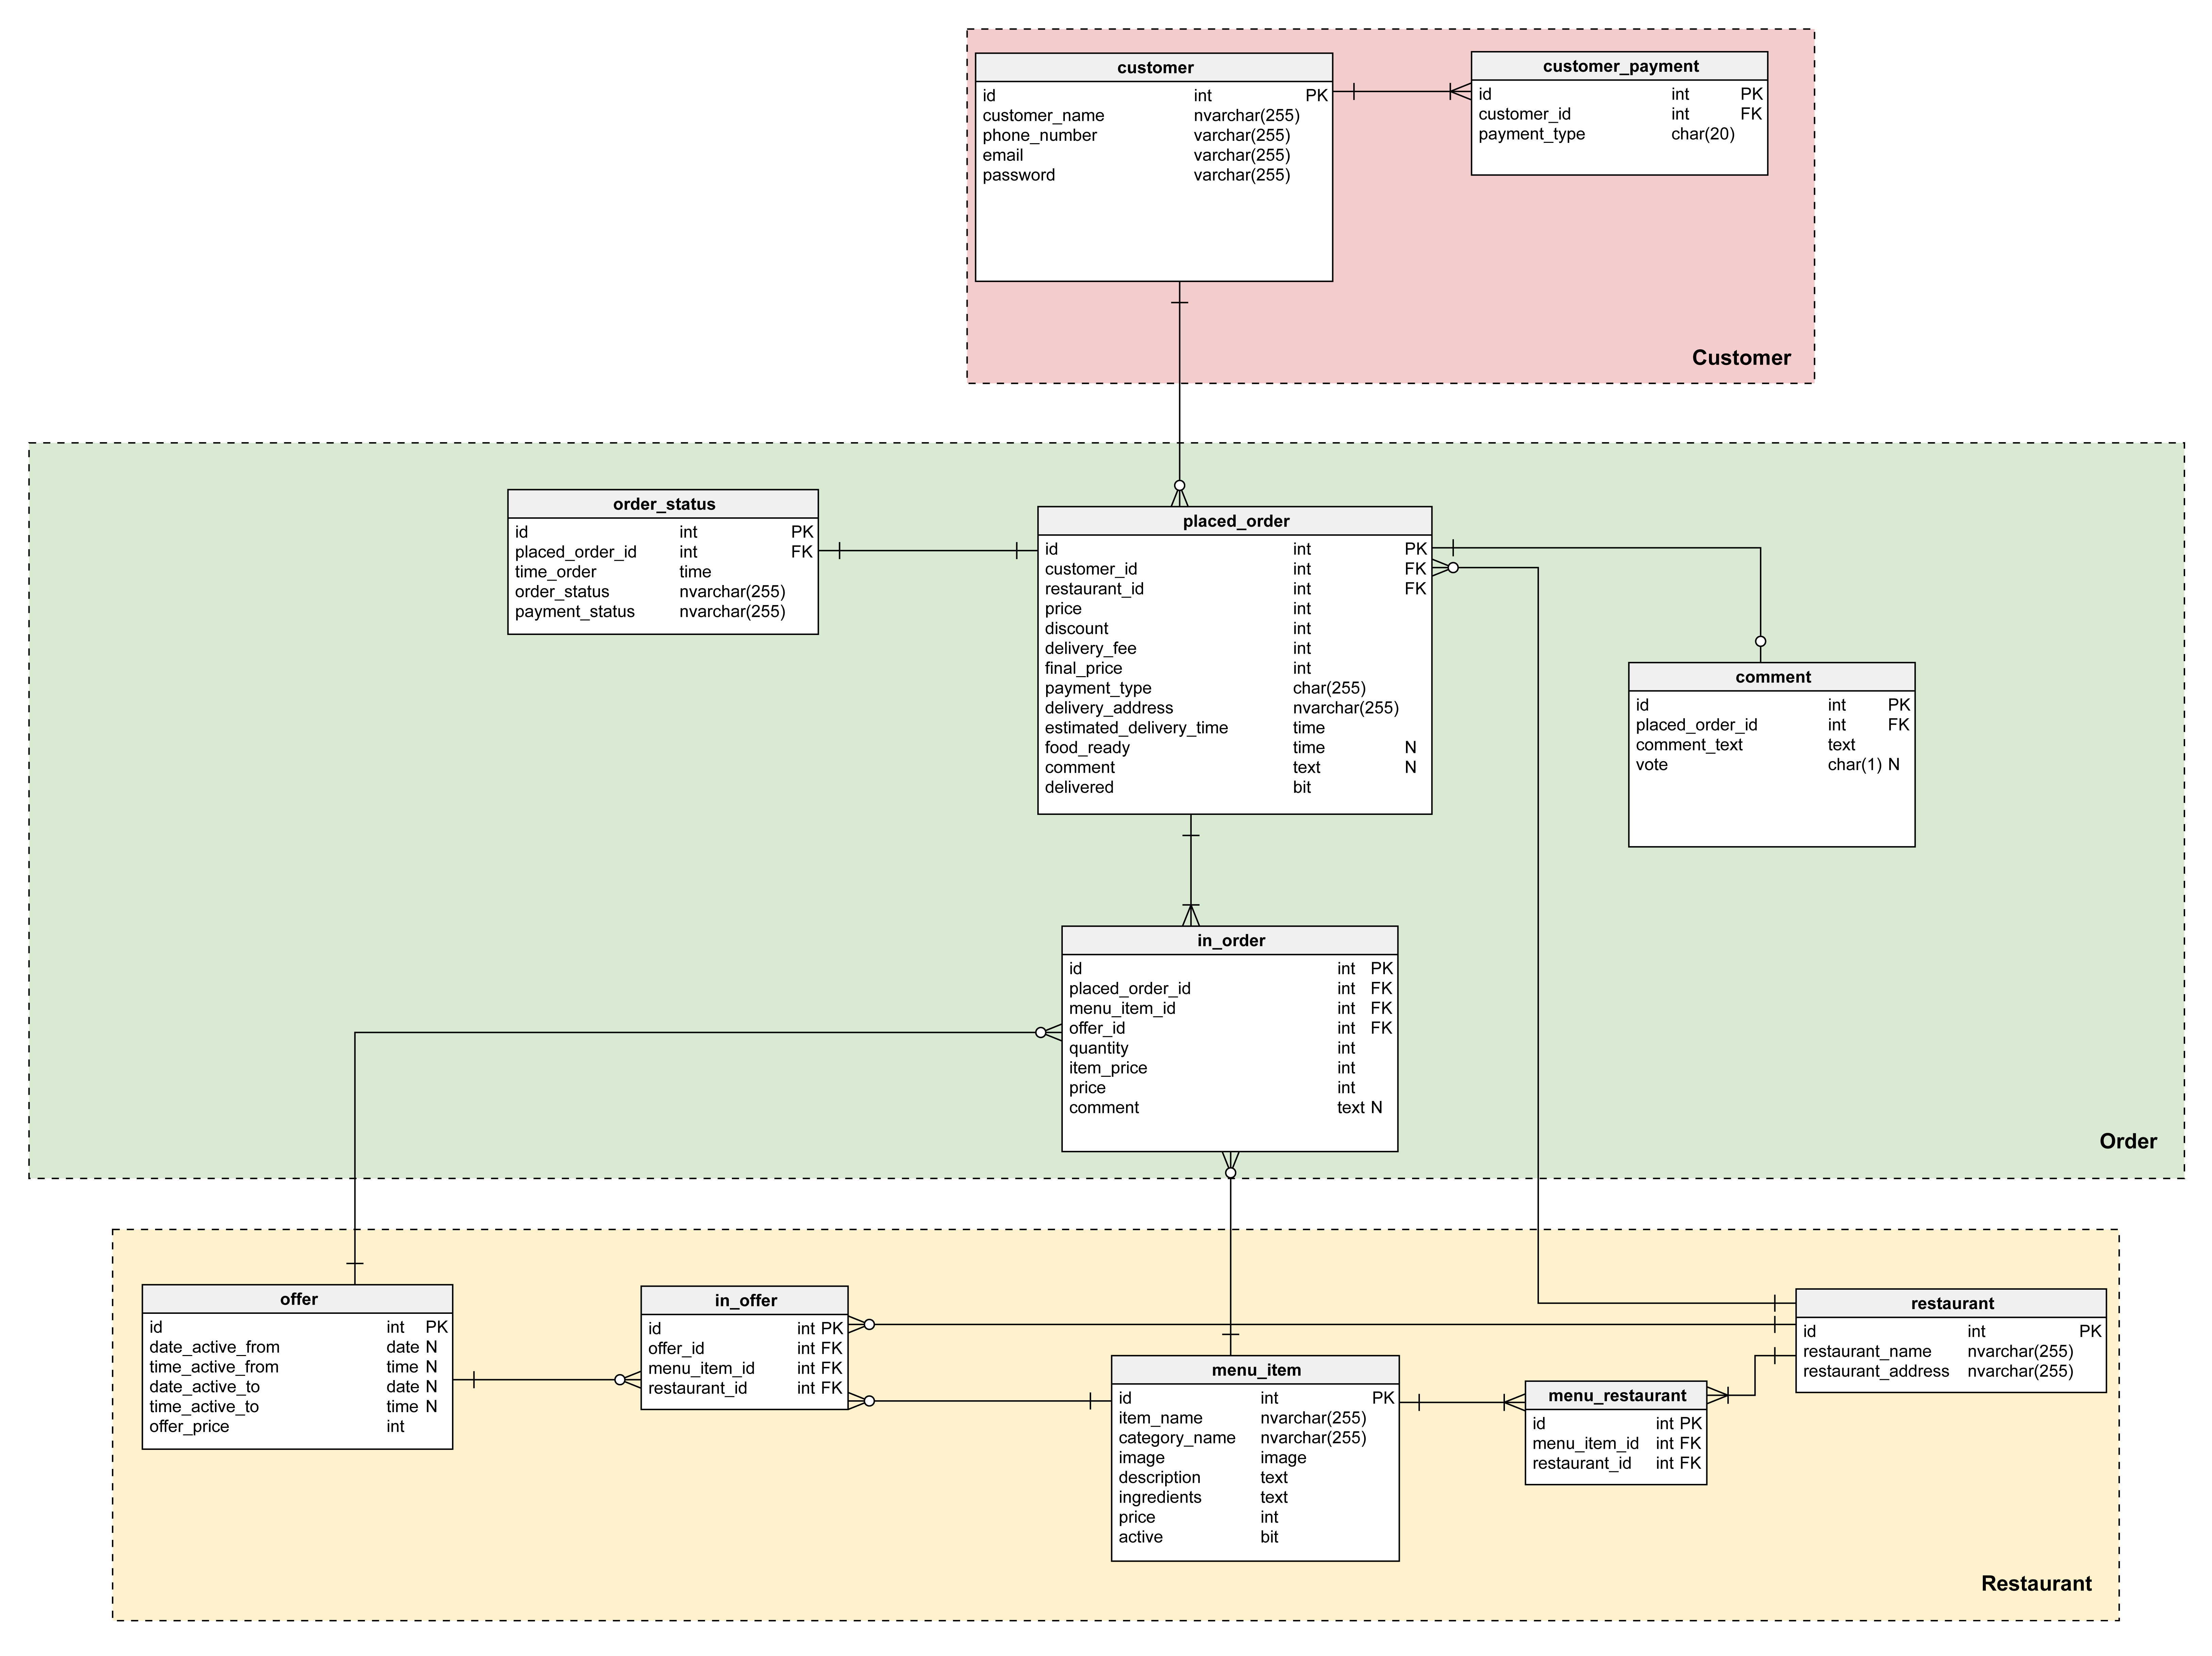
\includegraphics[width=0.9\textwidth]{sql_1.png}}
			\label{fig:ass1}
		\end{figure}
	\end{frame}
	\begin{frame}{Các thành phần chính}
		\tableofcontents
	\end{frame}
	\section{Customer}
	\begin{frame}
		\textcolor{structure}{\Huge{\textbf{Customer}}}
	\end{frame}
	%------------------------------------------------
	\begin{frame}{Customer}
		\begin{figure}[ht!]
			\centerline{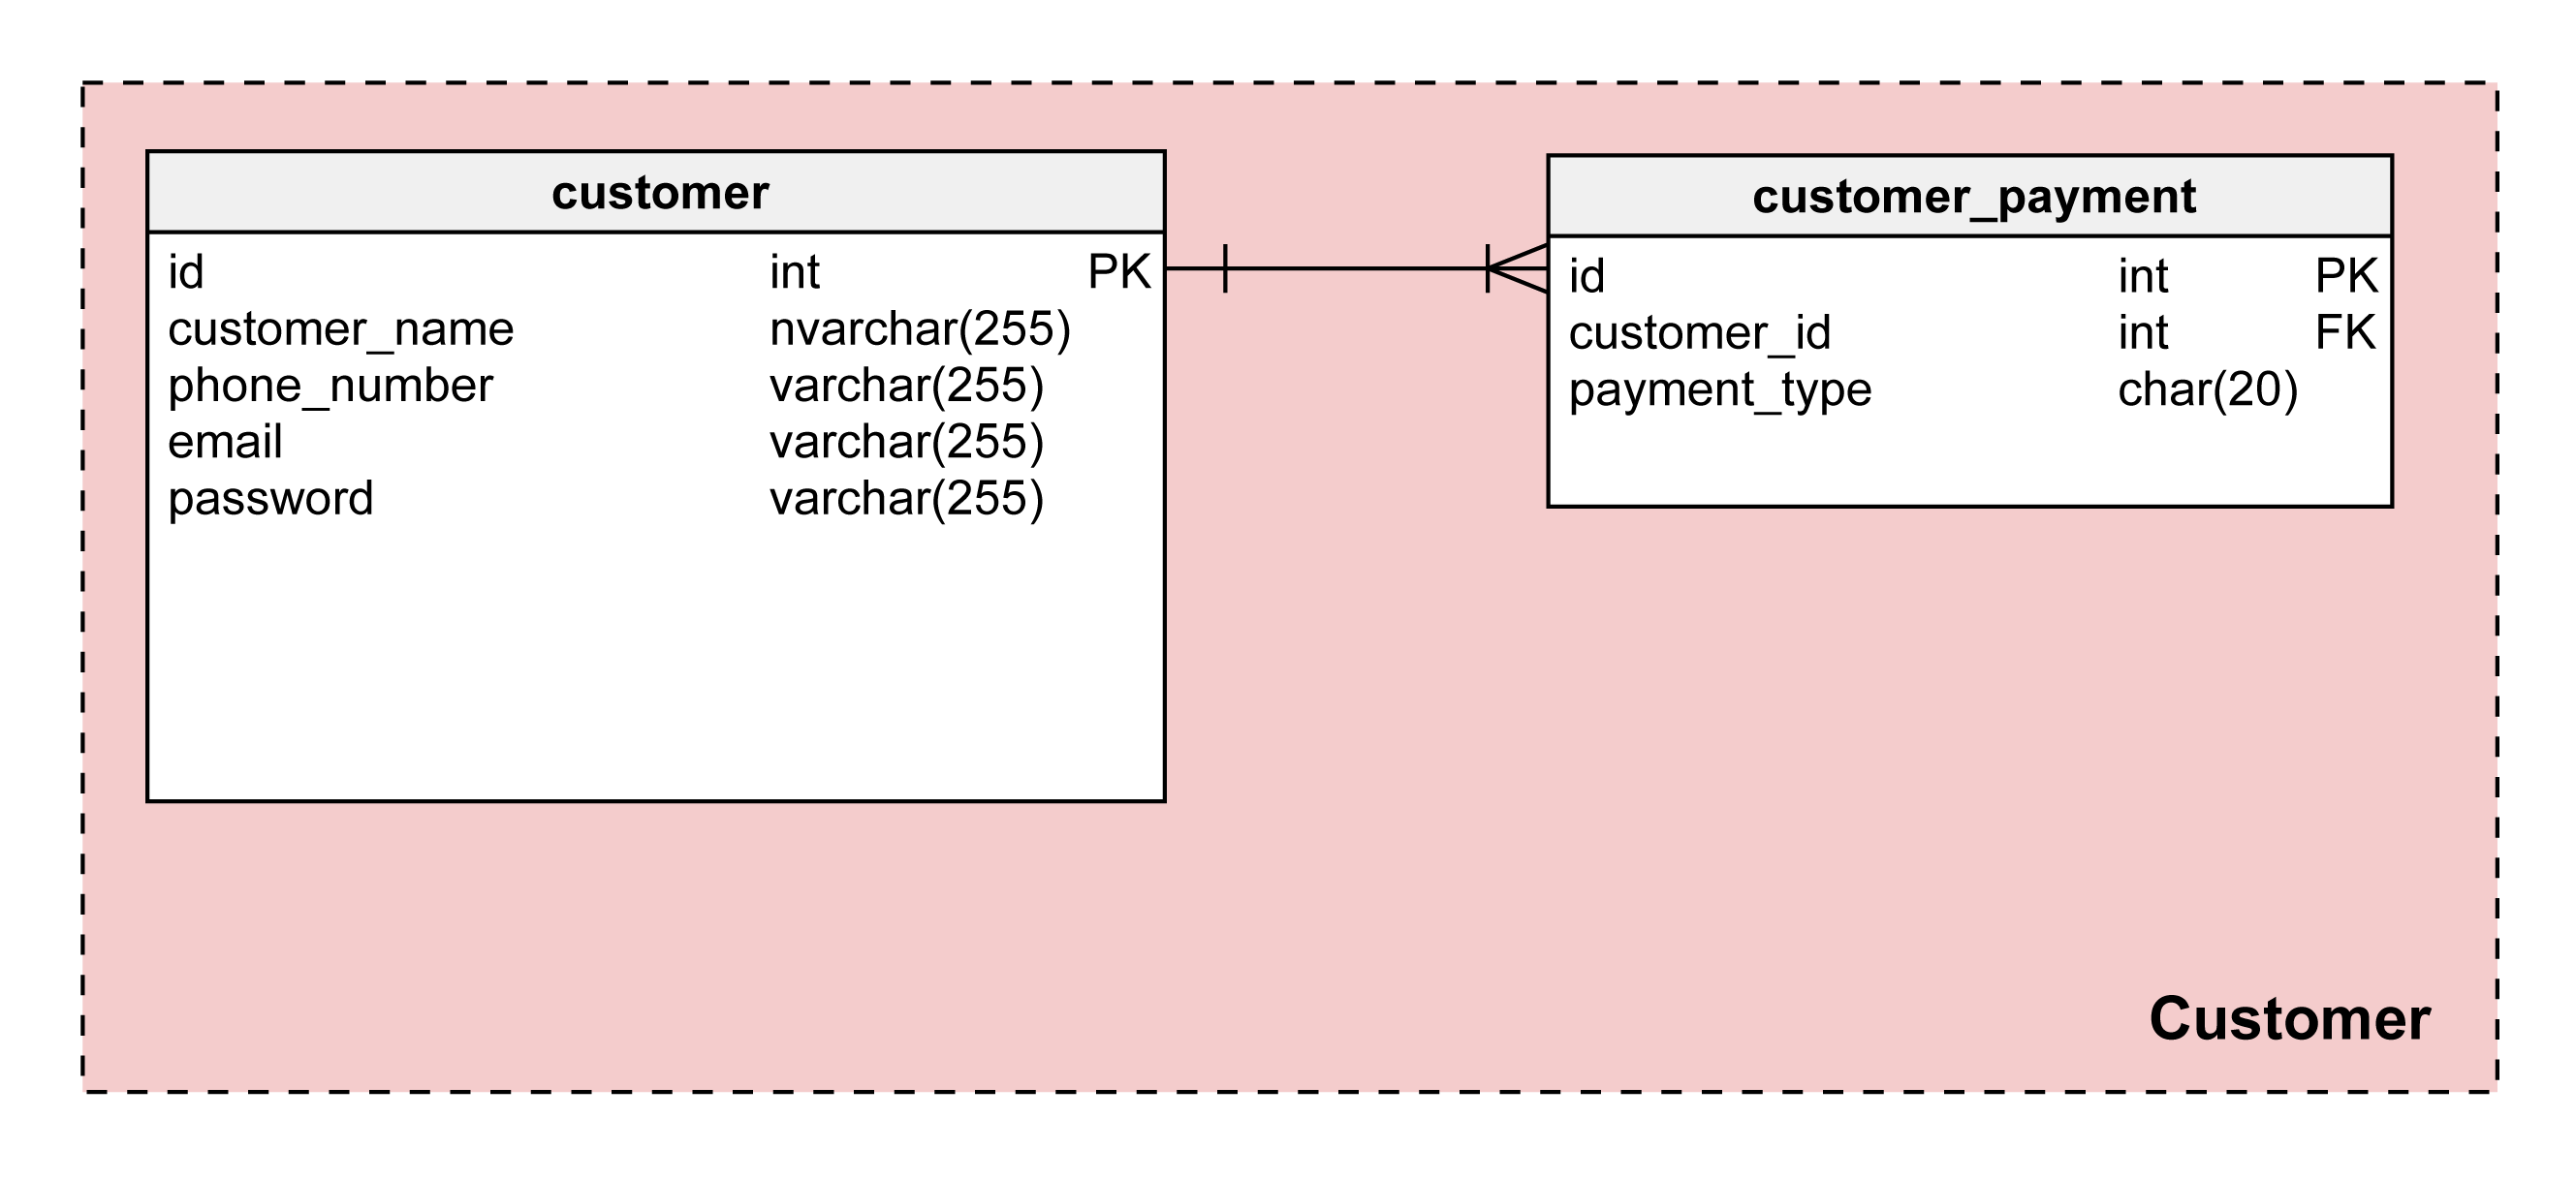
\includegraphics[width=1\textwidth]{customer.png}}
			\label{fig:ass1}
		\end{figure}
	\end{frame}
	\begin{frame}{Customer}
		\textcolor{structure}{\large{\textbf{Customer:}}}
		\begin{itemize}
			\item \textbf{id:} Mã khách hàng (Primary key)
			\item \textbf{customer$\_$name:} Tên khách hàng
			\item \textbf{phone$\_$number:} Số điện thoại khách hàng
			\item \textbf{email:} Mail khách hàng
			\item \textbf{password:} Mật khẩu tài khoản
		\end{itemize}
		\textcolor{structure}{\large{\textbf{Customer\_payment}}}
		\begin{itemize}
			\item \textbf{id:} (Primary key)
			\item \textbf{customer\_id:} Foreign key customer(id)
			\item \textbf{payment\_type:} Phương thức thanh toán
		\end{itemize}
	\end{frame}
	\section{Order}
	\begin{frame}
		\textcolor{structure}{\Huge{\textbf{Order}}}
	\end{frame}
	\begin{frame}{Order}
		\begin{figure}[ht!]
			\centerline{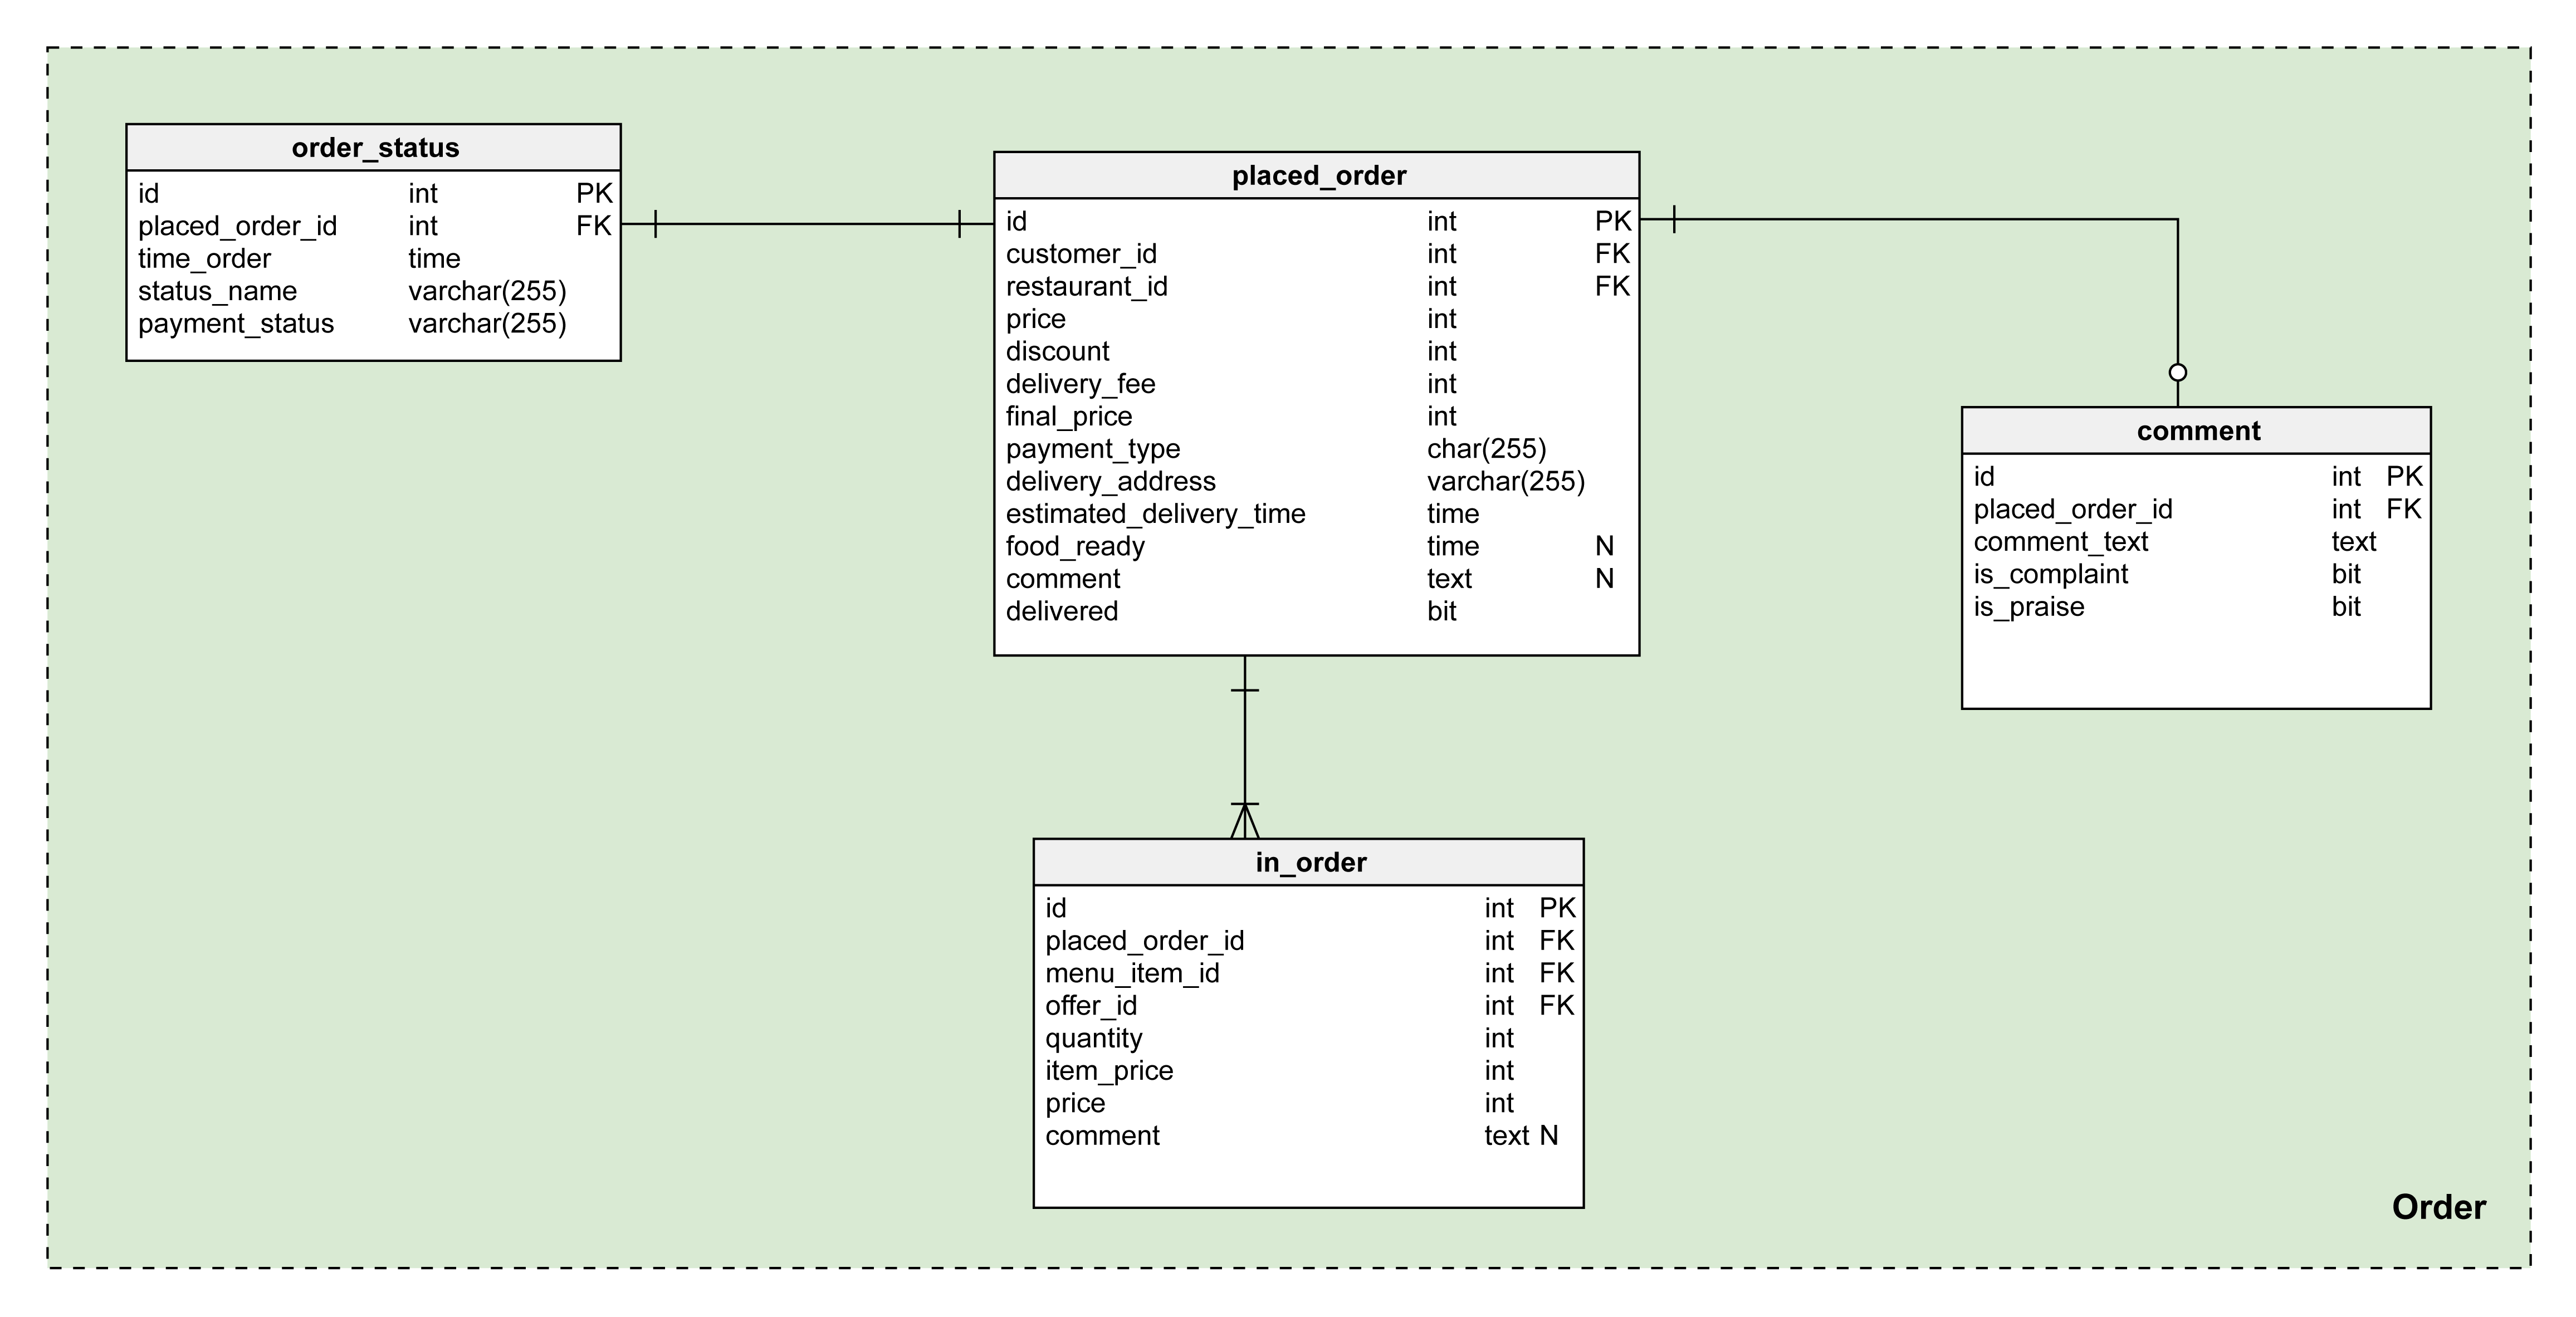
\includegraphics[width=1\textwidth]{order.png}}
			\label{fig:ass1}
		\end{figure}
	\end{frame}
	\begin{frame}{Placed Order}
		\begin{itemize}
			\item \textbf{id:}
			\item \textbf{customer\_id:} Foreign key customer(id)
			\item \textbf{restaurant\_id:} Foreign key restaurant(id)
			\item \textbf{price:} Giá ban đầu
			\item \textbf{discount:} Giảm giá 
			\item \textbf{delivery\_fee: }Phí vận chuyển
			\item \textbf{final\_price:} Giá phải trả
			\item \textbf{payment\_type:} Hình thức thanh toán
			\item \textbf{delivery\_address:} Địa chỉ giao hàng 
			\item \textbf{estimated\_delivery\_time:} Thời gian dự kiến giao hàng
			\item \textbf{food\_ready:} Đồ ăn đã sẵn sàng chưa
			\item \textbf{comment:} Lưu ý của khách hàng
			\item \textbf{deliveried:} Đã được giao hay chưa
		\end{itemize}
	\end{frame}
	
	\begin{frame}{Order status}
		\begin{itemize}
			\item \textbf{id:} Mã trạng thái đơn hàng
			\item \textbf{placed\_order\_id:} Mã đơn đặt hàng (Foreign key placed\_order(id))
			\item \textbf{time\_order:} Thời gian đặt hàng
			\item \textbf{status\_name:} Trạng thái đơn hàng (Thêm vào giỏ/ Xác nhận/ Đã thanh toán / Đã giao)
			\item \textbf{payment\_status:} Trạng thái thanh toán
		\end{itemize}
	\end{frame}
	
	\begin{frame}{In order}
		\begin{itemize}
			\item \textbf{id:} Mã
			\item \textbf{placed\_order\_id:} Mã đơn đặt hàng (Foreign key placed\_order(id))
			\item \textbf{offer\_id:} Mã ưu đãi (Foreign key offer(id))
			\item \textbf{menu\_item\_id:} Mã mặt hàng (Foreign key menu\_item(id))
			\item \textbf{quantity:} Số lượng mua
			\item \textbf{item\_price:} Giá lẻ
			\item \textbf{price:} Tổng giá
			\item \textbf{Comment:} Lưu ý của khách hàng (giao 11h30 chả hạn)
		\end{itemize}
	\end{frame}
	
	\begin{frame}{Comment}
		\begin{itemize}
			\item \textbf{id:}
			\item \textbf{placed\_order\_id:} Mã đơn đặt hàng (Foreign key placed\_order(id))
			\item \textbf{customer\_id:} Mã khách hàng (Foreign key customer(id))
			\item \textbf{comment\_text:} Đánh giá của khách hàng
			\item \textbf{is\_complaint:} Có phải lời phàn nàn không?
			\item \textbf{is\_complaint:} Có phải lời khen không?
		\end{itemize}
	\end{frame}
	\section{Restaurant}
	\begin{frame}
		\textcolor{structure}{\Huge{\textbf{Restaurant}}}
	\end{frame}
	\begin{frame}{Restaurant}
		\begin{figure}[ht!]
			\centerline{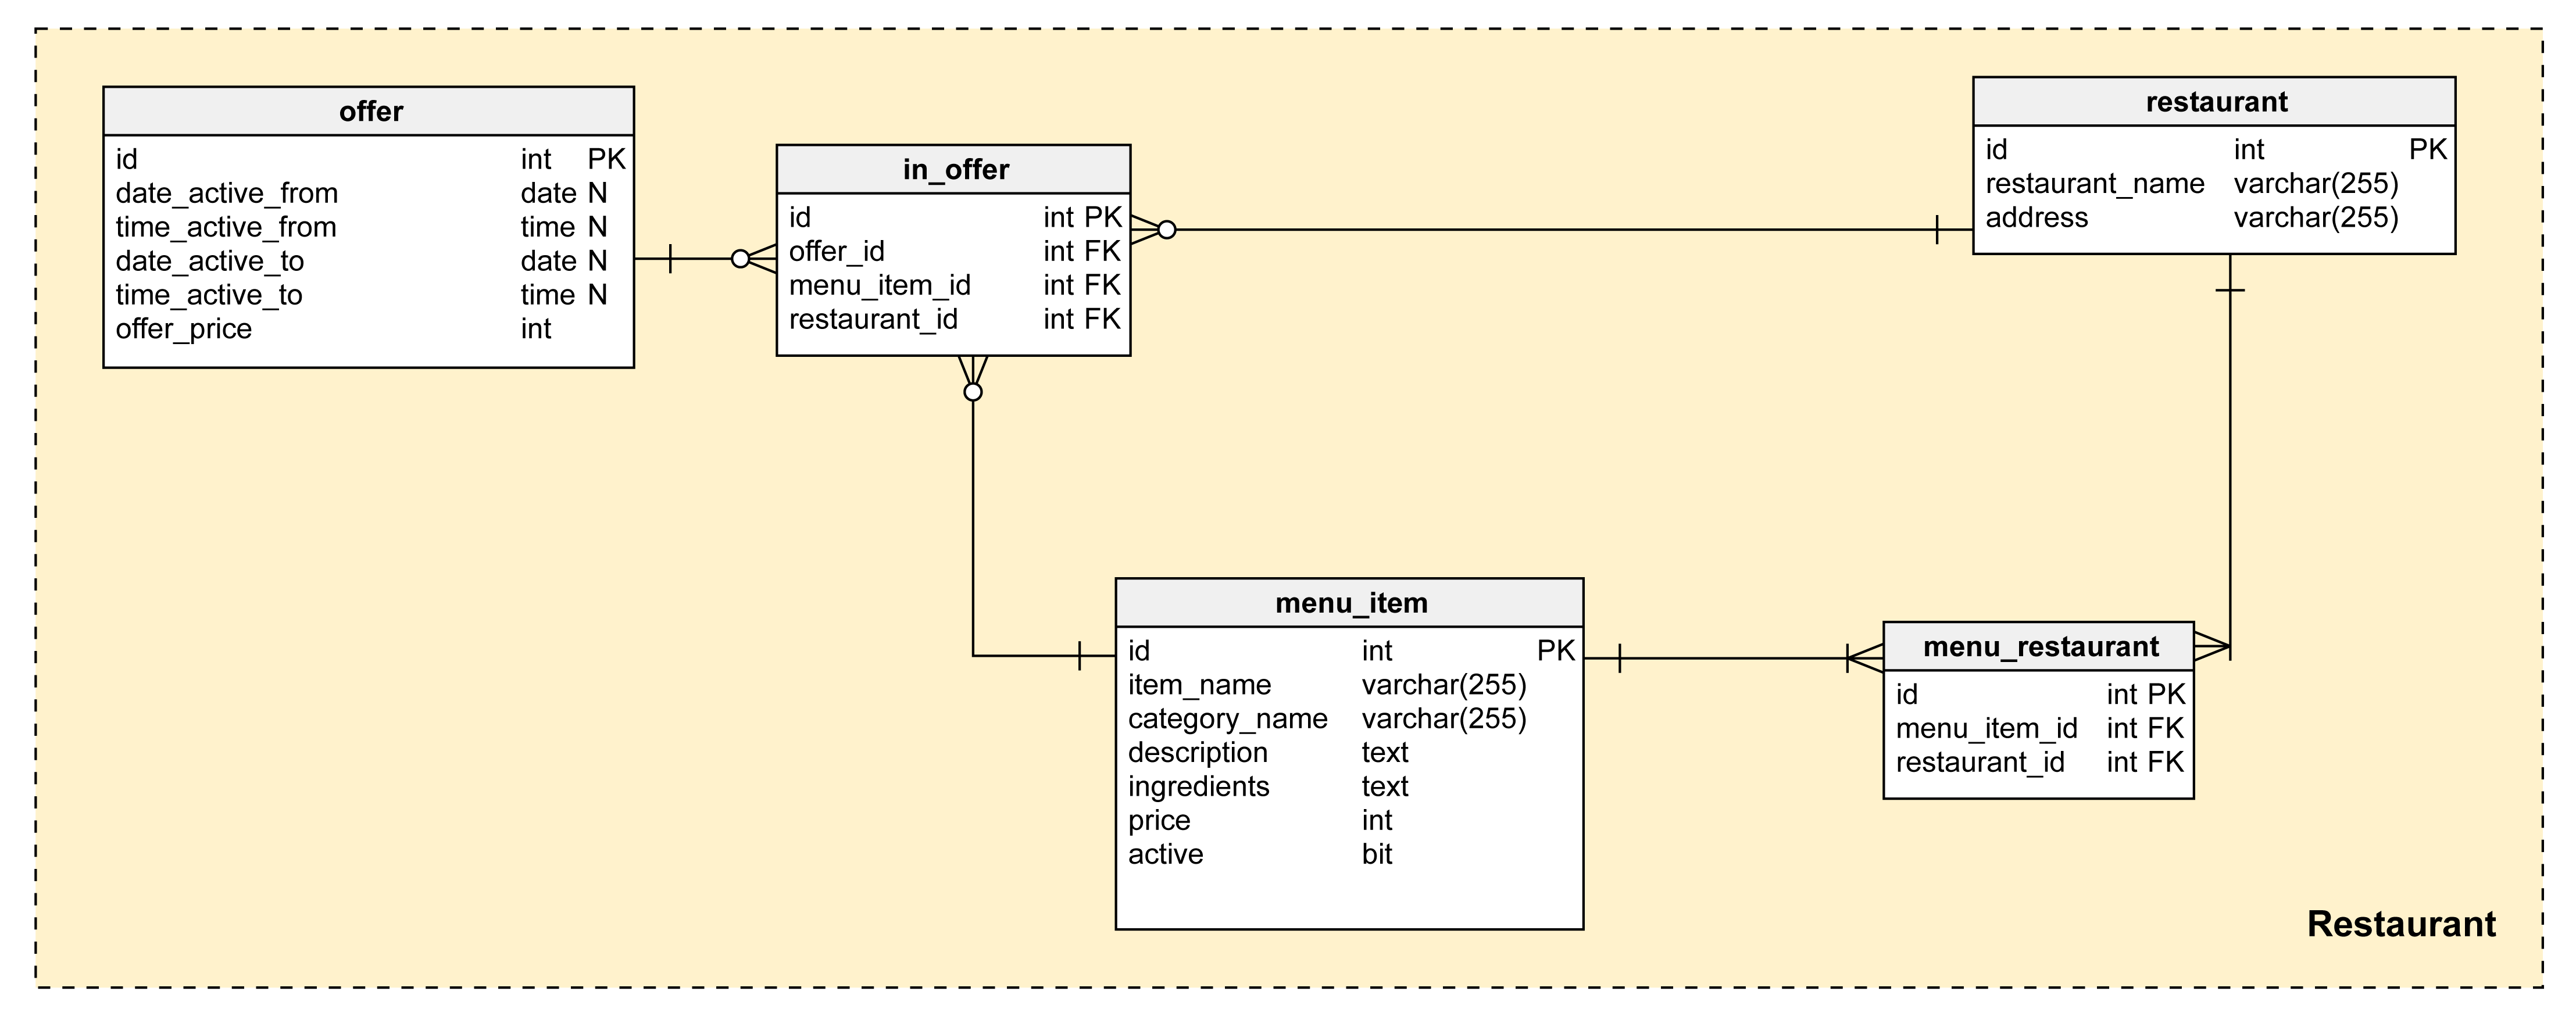
\includegraphics[width=1\textwidth]{restaurant.png}}
			\label{fig:ass1}
		\end{figure}
	\end{frame}
	\begin{frame}{Menu item}
		\begin{itemize}
			\item \textbf{id:} Mã món ăn (Primary key)
			\item \textbf{item\_name:} Tên món ăn
			\item \textbf{category\_name:} Phân loại
			\item \textbf{description:} Mô tả
			\item \textbf{ingredients:} Nguyên liệu
			\item \textbf{price:} Giá
			\item \textbf{active:} Tình trạng mặt hàng (còn hay hết)
		\end{itemize}
	\end{frame}
	
	\begin{frame}{Restaurant}
		\begin{itemize}
			\item \textbf{id: } Mã nhà hàng
			\item \textbf{restaurant\_name:} Tên nhà hàng
			\item \textbf{address:} Địa chỉ
		\end{itemize}
	\end{frame}
	
	\begin{frame}{Menu restaurant}
		%Lưu thông tin thực đơn của các nhà hàng (món ăn nào thuộc nhà hàng nào)
		\begin{itemize}
			\item \textbf{id: } Mã
			\item \textbf{menu\_item\_id: } Foreign key menu\_item(id)
			\item \textbf{restaurant\_id: } Foreign key restaurant(id)
		\end{itemize}
	\end{frame}
	
	\begin{frame}{Offer}
		\begin{itemize}
			\item \textbf{id: } Mã ưu đãi
			\item \textbf{data\_active\_from:} Ngày bắt đầu kích hoạt
			\item \textbf{time\_active\_from:} Giờ bắt đầu kích hoạt
			\item \textbf{data\_active\_to:} Ngày kết thúc kích hoạt
			\item \textbf{time\_active\_to:} Giờ kết thúc kích hoạt
			\item \textbf{offer\_price:} Giá trị ưu đãi
		\end{itemize}
	\end{frame}
	\begin{frame}{In offer}
		%Lưu thông tin giảm giá với mặt hàng tương ứng (sale thì mỗi mặt hàng 1 kiểu)
		\begin{itemize}
			\item \textbf{id: } Mã
			\item \textbf{offer\_id: } Foreign key offer(id)
			\item \textbf{menu\_item\_id: } Foreign key menu\_item(id)
			\item \textbf{restaurant\_id: } Foreign key restaurant(id)
		\end{itemize}
	\end{frame}

	
	
	\begin{frame}
		\Huge{\centerline{\textbf{The End}}}
	\end{frame}
	
	%----------------------------------------------------------------------------------------
	
\end{document}